\chapter{Proposta}
\label{chapter:proposal}

Conforme apresentado no \autoref{chapter:introduction}, a duplicação do código de configuração de acessórios prejudica a manutenibilidade dos testes, mas sua remoção manual torna-se progressivamente mais difícil à medida que a suíte cresce. O problema não se limita a identificar trechos repetidos: também é necessário decidir como redistribuir os métodos entre classes de teste sem aumentar o esforço total de desenvolvimento e manutenção e sem alterar o resultado observado dos testes.

O objetivo da proposta consiste em reduzir essa duplicação agrupando, em uma mesma classe, testes que possuam a mesma sequência inicial de configuração de acessórios. O código comum pode, então, ser extraído para um método de configuração executado antes de cada teste e reusado por meio da estratégia de configuração implícita. Dessa forma, cada método mantém apenas a configuração que lhe é específica, enquanto a classe centraliza a parte compartilhada por todos os seus testes.

Essa distribuição não é tratada como uma sucessão de decisões locais, nas quais se escolhe isoladamente uma classe para cada novo teste. A movimentação de um teste pode alterar tanto o código reusável quanto a duplicação introduzida nos demais testes da classe. Por isso, este trabalho aborda a distribuição dos testes como um problema de otimização global sobre toda a suíte: busca-se uma organização em classes que reduza a duplicação total ao aumentar o reuso das sequências iniciais de configuração de acessórios, preservando o comportamento observado dos testes. A refatoração pode ser aplicada em qualquer momento da evolução da suíte. Assim, quando novos testes forem adicionados, o processo pode ser executado novamente para recalcular a distribuição global e incorporá-los à organização das classes.

Para operacionalizar essa abordagem, o trabalho contribui com (1) uma arquitetura em pipeline para refatoração de código de teste; e (2) o Róża, um framework extensível que instancia essa arquitetura. A arquitetura define as responsabilidades e o fluxo de dados da refatoração, enquanto o framework oferece componentes e pontos de extensão para concretizar esse fluxo. As seções seguintes apresentam esses dois elementos.

\section{Arquitetura em pipeline}
\label{section:pipeline-architecture}

A Figura~\ref{figure:pipeline-architecture} apresenta a arquitetura, que organiza o processo de refatoração em um pipeline de sete etapas: carregamento, análise sintática, decomposição, medição, agrupamento, refatoração e escrita. Cada etapa recebe os dados produzidos pela etapa anterior e gera a entrada da próxima. Essa separação permite substituir uma estratégia sem modificar as demais partes do processo. Assim, diferentes formas de obter os arquivos, linguagens, frameworks de teste, métricas de similaridade, algoritmos de agrupamento, estratégias de refatoração e destinos de escrita podem ser combinados dentro do mesmo fluxo. Embora o objetivo deste trabalho seja promover o reuso de código por meio da configuração implícita, a arquitetura não se restringe a essa estratégia. Sua flexibilidade permite incorporar outros tipos de refatoração, como a extração de código comum por meio da configuração delegada.

\begin{figure}[htb]
	\centering
	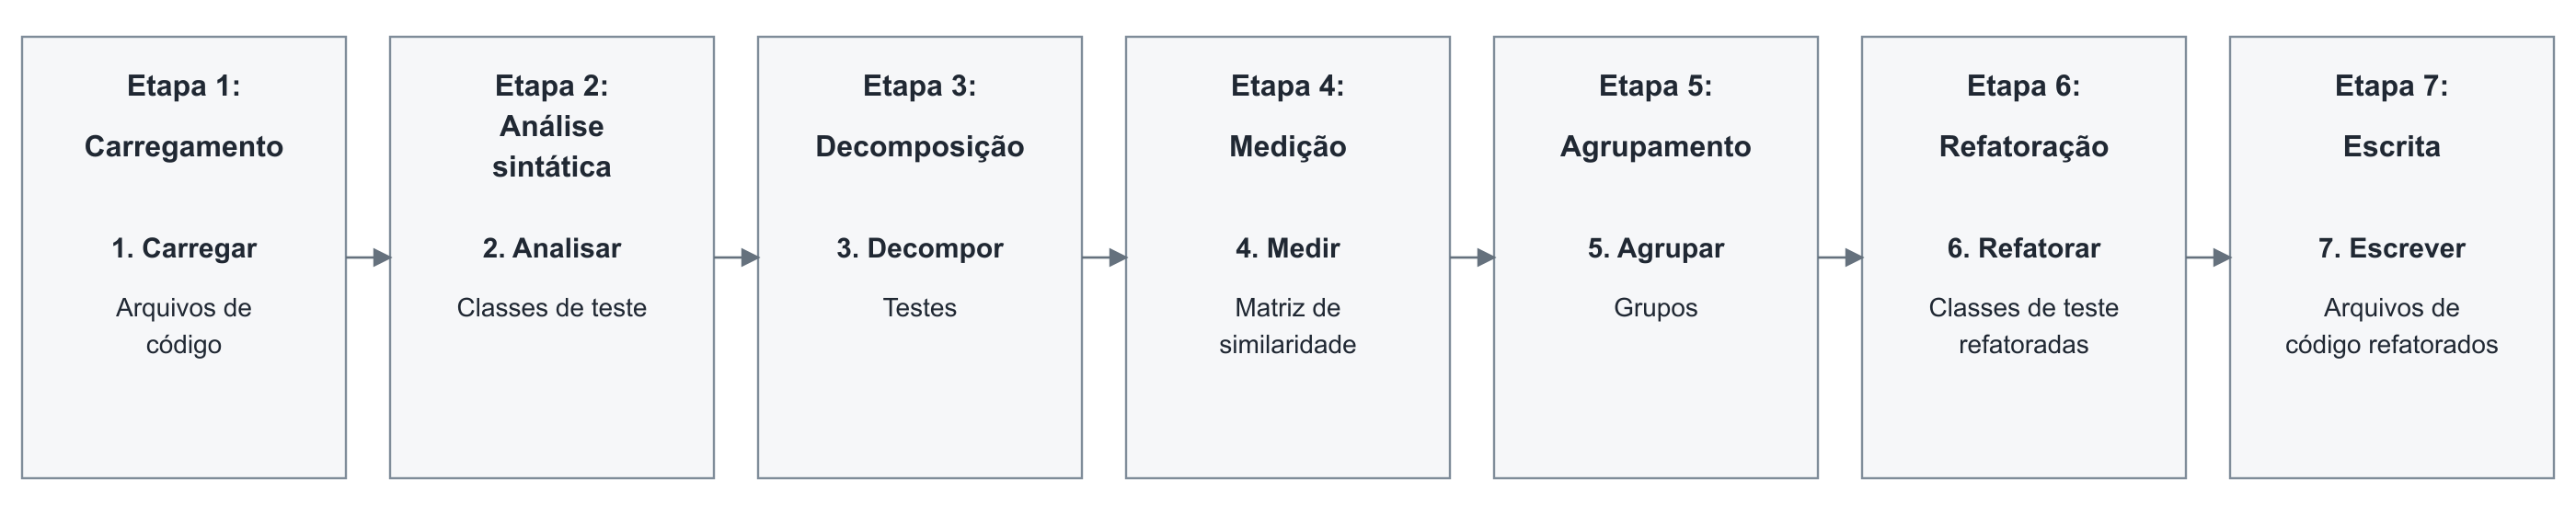
\includegraphics[width=\textwidth]{figures/pipeline-architecture.png}
	\caption{Arquitetura em pipeline para refatoração de código de teste}
	\label{figure:pipeline-architecture}
	\fonte{Elaborado pelo autor.}
\end{figure}

O fluxo de dados percorre as sete etapas na seguinte ordem: (1) o carregamento produz os arquivos de código; (2) a análise sintática identifica as classes de teste e as converte em um modelo estrutural em memória; (3) a decomposição produz uma representação individual de cada teste; (4) a medição produz a matriz de similaridade entre os testes; (5) o agrupamento produz grupos de testes; (6) a refatoração reconstrói as classes de teste a partir desses grupos; e (7) a escrita persiste os arquivos de código refatorados.

A primeira etapa, denominada \textbf{carregamento}, obtém os arquivos de código e os mantém em memória. Esses arquivos ainda não são interpretados como testes: o carregamento não identifica classes de teste nem constrói um modelo estrutural. Essa separação permite combinar diferentes estratégias de obtenção de arquivos (e.g., leitura recursiva do sistema de arquivos, filtro por extensão ou carregamento a partir de um repositório) com as etapas seguintes.

Na etapa de \textbf{análise sintática}, os arquivos carregados são examinados para identificar aqueles que contêm classes de teste. Cada classe identificada é convertida em uma árvore abstrata de sintaxe (\textit{Abstract Syntax Tree} -- AST), que representa sua estrutura em memória e permite identificar e manipular atributos, métodos de configuração e métodos de teste.

Na etapa de \textbf{decomposição}, cada teste é separado de sua classe de origem e associado a todo o código necessário para sua execução. A decomposição realiza, portanto, o movimento oposto ao da refatoração: em vez de agrupar testes e extrair o código comum, ela incorpora a cada teste a configuração da qual ele depende para isolá-lo de sua classe original. Isso inclui tanto a configuração declarada diretamente no método de teste quanto aquela proveniente de métodos de configuração implícita. O resultado é uma representação individual de cada teste, composta por sua configuração de acessórios, seu exercício e suas asserções. Esse isolamento permite que os testes sejam comparados individualmente na etapa de medição.

Na etapa de \textbf{medição}, consideram-se apenas as configurações de acessórios, pois são elas que contêm o código que se pretende reusar. A métrica calcula o grau de similaridade entre cada par de testes e produz uma matriz de similaridade. Quando a métrica opera sobre arquivos, a configuração de cada teste é materializada internamente nesta etapa, isto é, gravada em um arquivo separado. Métricas capazes de consumir a representação em memória dispensam essa materialização. A matriz reúne as relações entre todos os testes da suíte e constitui a entrada da etapa de agrupamento.

Na etapa de \textbf{agrupamento}, um algoritmo utiliza a matriz de similaridade para propor uma distribuição global dos testes. Cada grupo representa uma futura classe de teste. O objetivo não é apenas reunir os pares mais similares isoladamente, mas encontrar grupos cuja configuração inicial comum possibilite reduzir a duplicação total da suíte por meio da configuração implícita.

Na etapa de \textbf{refatoração}, as classes de teste são reconstruídas com base nos grupos propostos. Para cada grupo, cria-se uma classe, inserem-se os testes correspondentes e move-se a sequência inicial de configuração compartilhada por todos eles para um método de configuração implícita. A segurança dessa transformação depende de restringir os comandos extraídos. Move-se somente a sequência inicial comum a todos os testes do grupo, preservando a ordem relativa no método de configuração. A transformação assume a independência dos testes, discutida no \autoref{chapter:background}: os acessórios de um teste não devem depender da ordem de execução nem do estado residual deixado por outros testes. Como somente o código comum a todos os testes da classe é reusado por meio desse método, nenhum teste executa uma configuração da qual não necessita, o que pode mitigar o fedor de acessórios generalizados.

Por fim, a etapa de \textbf{escrita} persiste os arquivos de código refatorados em um destino de saída, como o sistema de arquivos. Com isso, o fluxo proposto se encerra em artefatos de código, e não apenas em um modelo em memória.

\section{Framework Róża}
\label{section:roza-framework}

O Róża é um framework extensível concebido para instanciar a arquitetura em pipeline e encontra-se em desenvolvimento. No estágio atual desta pesquisa, foi implementado o fluxo até a etapa de medição, compreendendo o carregamento, a análise sintática, a decomposição e a medição. Esse fluxo produz a matriz de similaridade necessária para a continuação do pipeline. As etapas de agrupamento, refatoração e escrita integram a arquitetura proposta, mas ainda não foram implementadas no framework. A Figura~\ref{figure:roza-class-diagram} apresenta as classes e as interfaces atualmente implementadas. Por concisão, o diagrama omite a maior parte das demais classes e apresenta apenas as principais.

\begin{figure}[htb]
	\centering
	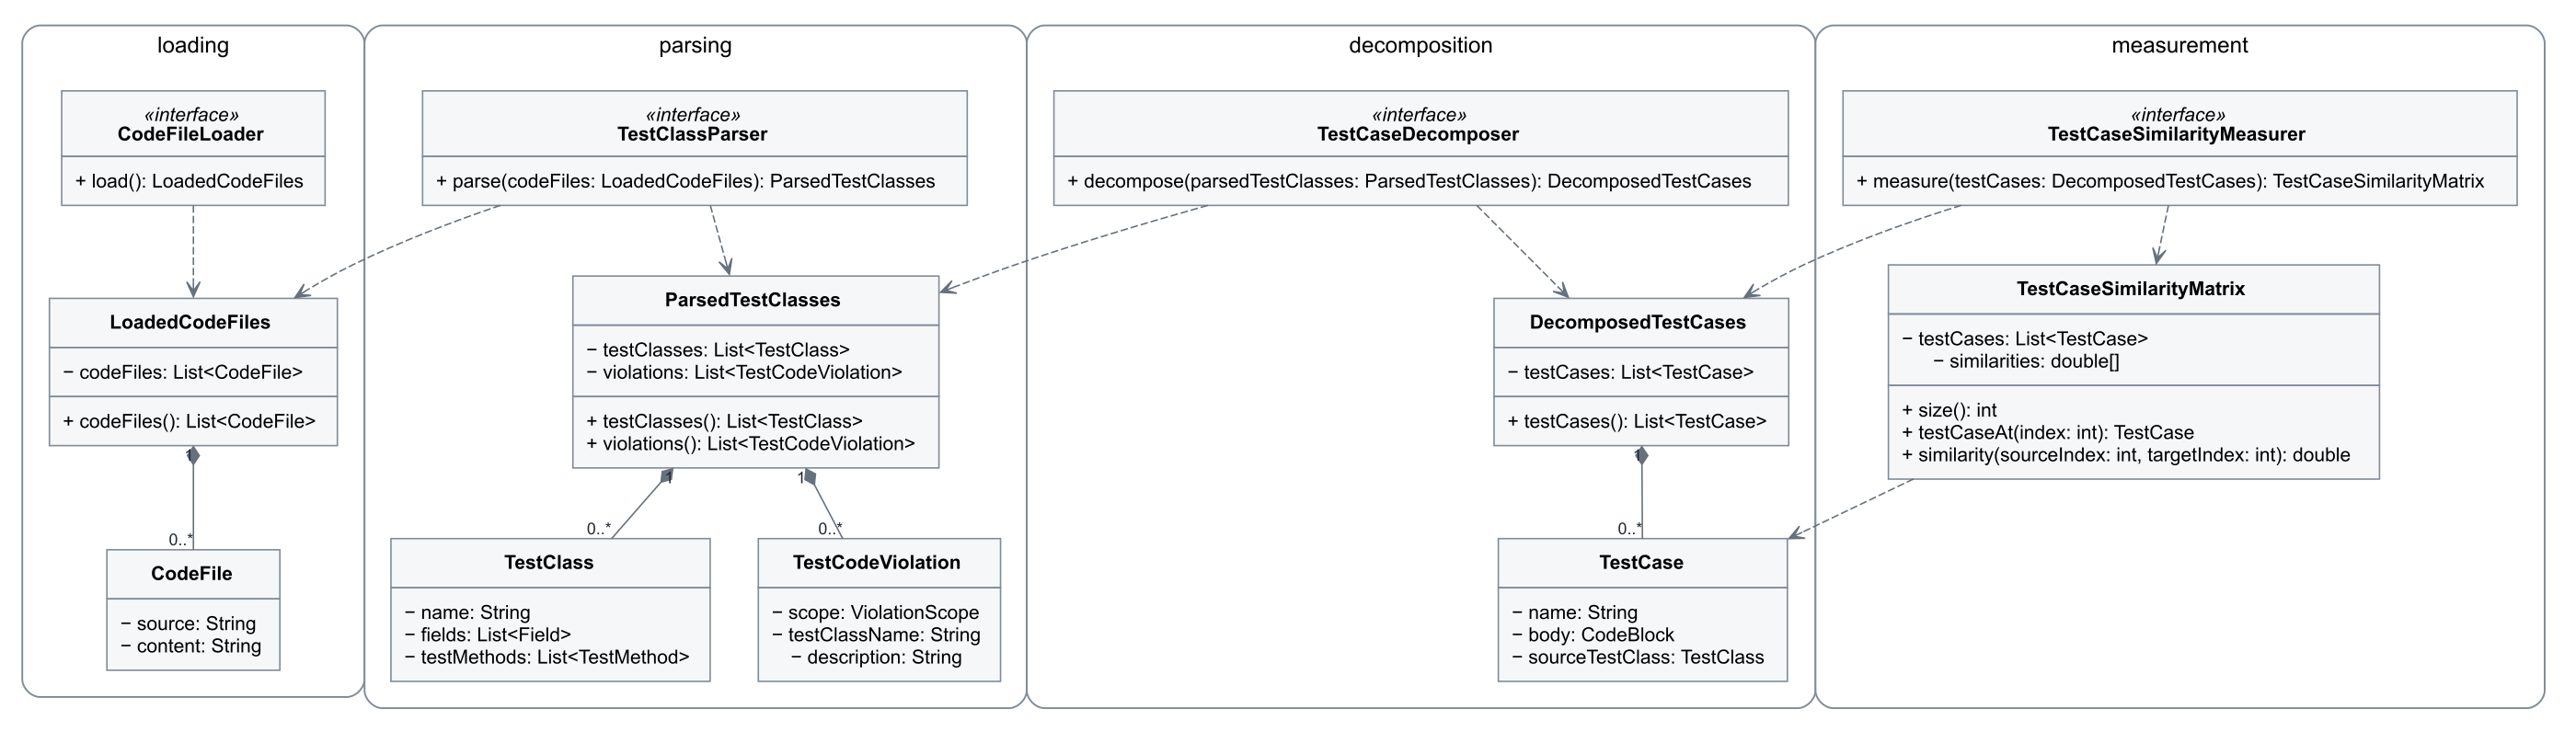
\includegraphics[width=\textwidth]{figures/roza-class-diagram.png}
	\caption{Diagrama de classes do Róża até a etapa de medição}
	\label{figure:roza-class-diagram}
	\fonte{Elaborado pelo autor.}
\end{figure}

As etapas implementadas correspondem às interfaces (1) \texttt{CodeFileLoader}, no carregamento; (2) \texttt{TestClassParser}, na análise sintática; (3) \texttt{TestCaseDecomposer}, na decomposição; e (4) \texttt{TestCaseSimilarityMeasurer}, na medição. Quando a métrica opera sobre arquivos, a materialização das configurações de acessórios ocorre internamente nessa última etapa.

Cada etapa é representada por um contrato de entrada e de saída, e não por uma implementação rígida. As implementações não se invocam mutuamente: um orquestrador consome o artefato produzido por uma etapa e o fornece à seguinte. Com isso, uma implementação de análise sintática pode ser combinada com diferentes implementações de medição sem que qualquer uma delas conheça a outra. Novas linguagens ou métricas de similaridade entram no fluxo pela substituição do contrato correspondente.

A Figura~\ref{figure:roza-screenshot} apresenta a interface gráfica do Róża durante a etapa de medição, na qual é possível selecionar uma métrica de similaridade e inspecionar a configuração de acessórios de cada teste decomposto.

\begin{figure}[htb]
	\centering
	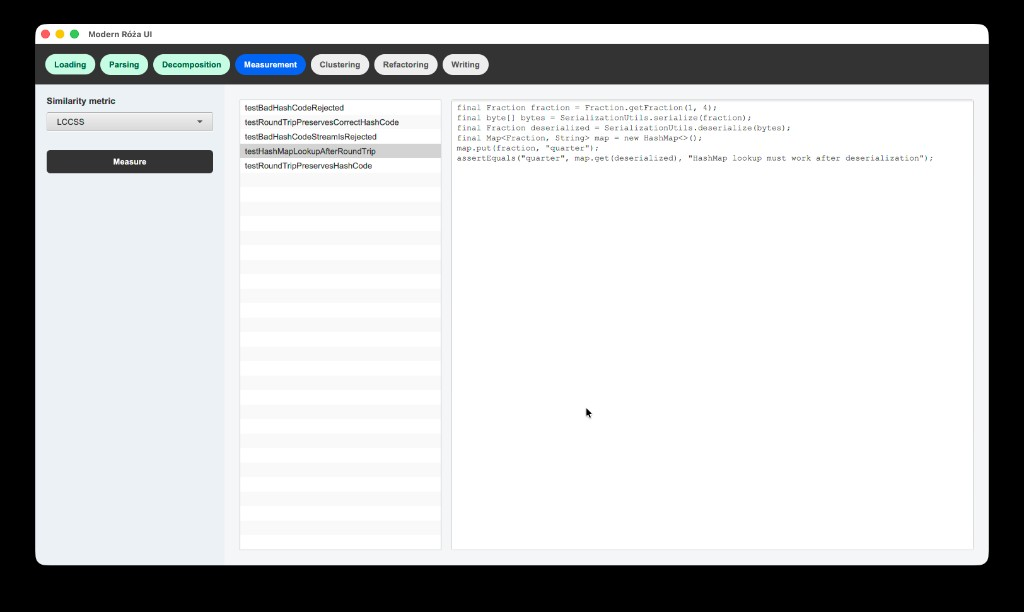
\includegraphics[width=\textwidth]{figures/roza-screenshot.png}
	\caption{Interface gráfica do Róża na etapa de medição}
	\label{figure:roza-screenshot}
	\fonte{Elaborado pelo autor.}
\end{figure}


A implementação atual processa classes de teste escritas em Java com o framework JUnit. A análise sintática dessas classes é realizada com a biblioteca JavaParser, da qual resulta o modelo estrutural utilizado nas etapas seguintes. Na medição, o framework oferece cinco métricas de similaridade: JPlag \cite{prechelt:etal:2002}, Simian, Deckard \cite{jiang:etal:2007}, a subsequência comum mais longa (\textit{Longest Common Subsequence} -- LCS) \cite{hirschberg:1977} e a subsequência comum inicial contígua mais longa (\textit{Longest Common Contiguous Start Subsequence} -- LCCSS) \cite{silva:etal:2020}. As seções seguintes apresentam cada uma dessas métricas.

\subsection{JPlag}
\label{subsection:jplag}

JPlag consiste em um detector de clones baseado em tokens, com suporte a linguagens como Java, C++ e Python \cite{prechelt:etal:2002}. A ferramenta admite um parâmetro de sensibilidade, correspondente ao número mínimo de tokens que devem coincidir para que um trecho seja considerado comum. No Róża, a configuração de acessórios de cada teste é materializada internamente em arquivos e a ferramenta é invocada. JPlag gera um relatório HTML e a implementação interpreta esse relatório para obter o grau de similaridade de cada par e registrá-lo na matriz de similaridade.

\subsection{Simian}
\label{subsection:simian}

Simian consiste em um detector de clones baseado em texto, aplicável a linguagens como Java, C++, C\# e Ruby. A ferramenta produz um relatório dos fragmentos considerados clones, e não um grau de similaridade. Por isso, o Róża interpreta esse relatório e calcula o grau de similaridade conforme a Equação~\ref{equation:simian-deckard-similarity}, definida como a razão entre o tamanho total dos fragmentos clonados, medido em linhas, e o tamanho do teste de origem \cite{ragkhitwetsagul:etal:2018}. Como os testes podem ter tamanhos distintos, a métrica é assimétrica (i.e., $\delta(\alpha, \beta)$ pode diferir de $\delta(\beta, \alpha)$). Fragmentos sobrepostos são unidos para que não sejam contados mais de uma vez. Simian admite um limiar correspondente ao número mínimo de linhas semelhantes, que deve ser um inteiro positivo com valor mínimo 2. Assim como em JPlag, a configuração de acessórios é materializada internamente em arquivos.

\begin{equation}
	\label{equation:simian-deckard-similarity}
	\delta(\alpha, \beta) = \frac{\sum_{i=1}^{n} \left|\mathrm{FRAGMENT}_{i}^{\alpha}(\alpha, \beta)\right|}{\left|\alpha\right|}
\end{equation}

\subsection{Deckard}
\label{subsection:deckard}

Deckard consiste em um detector de clones baseado em árvores \cite{jiang:etal:2007}. Assim como Simian, a ferramenta produz um relatório de clones, e o grau de similaridade é obtido pela Equação~\ref{equation:simian-deckard-similarity}, o que também torna a métrica assimétrica. Deckard oferece três parâmetros: o número mínimo de tokens para classificar dois fragmentos como clones; o passo (\textit{stride}), que indica quantos tokens podem ser ignorados ao unir fragmentos não contíguos; e o limiar mínimo de similaridade, com valores entre 0,0 e 1,0. A materialização das configurações de acessórios em arquivos ocorre internamente.

\subsection{LCS}
\label{subsection:lcs}

A LCS não é, em si, uma métrica de similaridade, mas uma sequência obtida a partir de outras duas, contendo os elementos comuns e preservando a ordem original \cite{hirschberg:1977}. No Róża, cada teste é representado por uma sequência de comandos da configuração de acessórios, e o grau de similaridade é calculado pela Equação~\ref{equation:lcs-similarity} \cite{dice:1945}. A métrica é simétrica e não exige configuração. Diferentemente de JPlag, Simian e Deckard, a LCS consome a representação em memória e dispensa a materialização em arquivos.

\begin{equation}
	\label{equation:lcs-similarity}
	\delta(\alpha, \beta) = \frac{\left|LCS(\alpha, \beta)\right| \times 2}{\left|\alpha\right| + \left|\beta\right|}
\end{equation}

\subsection{LCCSS}
\label{subsection:lccss}

A subsequência comum inicial contígua mais longa (\textit{Longest Common Contiguous Start Subsequence} -- LCCSS) foi inspirada na LCS e proposta neste trabalho para contornar limitações dessa métrica quando o objetivo é refatorar testes por meio da configuração implícita \cite{silva:etal:2020}. A LCS não penaliza comandos intercalados e pode atribuir grau elevado a testes cujos comandos iniciais diferem. Na extração para o método de configuração, apenas a sequência inicial comum pode ser movida. A LCCSS atribui grau elevado a testes cuja sequência inicial coincide. A Equação~\ref{equation:lccss-similarity} assemelha-se à da LCS, da qual a LCCSS é uma especialização. Assim como a LCS, a LCCSS não exige configuração e opera sobre a representação em memória.

\begin{equation}
	\label{equation:lccss-similarity}
	\delta(\alpha, \beta) = \frac{\left|LCCSS(\alpha, \beta)\right| \times 2}{\left|\alpha\right| + \left|\beta\right|}
\end{equation}
